\documentclass{article}
\usepackage{amsthm,thmtools,amsmath,amssymb}
\usepackage{graphicx}
\graphicspath{ {./images/} }
\usepackage{tkz-euclide}
\title{My Shool Geometry Notes}
\author{@mb6ockatf}
\date{\today}
\newtheorem{theorem}{Theorem}

\begin{document}
\maketitle
\tableofcontents

If hights of 2 triangles are equal, then their S correlate like their bases

\section{Triangle: Radius of Interior Circle}
$r = \frac{S_{ABC}}{0.5P}$
$$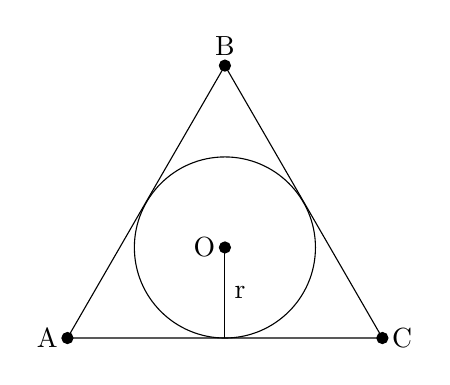
\begin{tikzpicture}
    \draw (0,0) -- (4,0) -- (2,3.46) -- cycle;
    \draw (2,1.15) circle (1.15);
    \filldraw[black] (2,1.15) circle (2pt) node[anchor=east]{O};
    \draw (2,1.15) -- (2,0);
    \filldraw[black] (2,0.575) circle (0pt) node[anchor=west]{r};
    \filldraw[black] (0,0) circle (2pt) node[anchor=east]{A};
    \filldraw[black] (2,3.46) circle (2pt) node[anchor=south]{B};
    \filldraw[black] (4,0) circle (2pt) node[anchor=west]{C};
\end{tikzpicture}$$

\section{Triangle: Egyptian Edition}
Triangles with such sides are right, i.e. have an angle of 90$^{\circ}$:\\

[3, 4, 5], [5, 12, 13], [8, 15, 17], [7, 24, 25], [20, 21, 29], [9, 40, 41]

\section{Tangent \& secant}
\begin{theorem}[Tangent and Secant]
If a tangent segment and a secant segment are drawn to a circle from an
exterior point, then the square of the measure of the tangent segment is
equal to the product of the measures of the secant segment and its external
secant segment.
\end{theorem}
\begin{proof}
	From similiarity of triangles:\\
	\includegraphics{tangent_n_secant.jpg}\\
	$\triangle{MCA} \sim \triangle{MBC}$ by 2 angles ($\angle{MCA} =
	\angle{ABC} = \phi$, $\angle{BMC}$ is common). $\implies$
	$\frac{MC}{MB} = \frac{MA}{MC}$, $MC^2 = MA * MB$
\end{proof}
\begin{theorem}[Two Secants (Secant Power)]
	When two secants intersect at an exterior point, the product of the
	one whole secant segment and its external segment is equal to the
	product of the other whole secant segment and its external segment\\
	\includegraphics{2secants}\\
	$MA * MB = MC * MD$
\end{theorem}
\begin{proof}
	$\triangle{MDA} \sim \triangle{MBC}$ by 3 angles, $\implies MA * MB = MC * CD$
\end{proof}

\section{Polygon}
\begin{theorem}[Sum of angles in polygon]
	Sum of angles in n-angled polygon equals to $(n - 2) * 180$
\end{theorem}
\end{document}
